\documentclass[]{scrartcl}

\usepackage{geometry}
\geometry{a4paper,left=25mm,right=25mm, top=1cm, bottom=2cm} 
\usepackage[latin1]{inputenc}
\usepackage{amsmath}
\usepackage{amsfonts}
\usepackage{amssymb}
\usepackage{graphicx}
%\usepackage{subfig}
\usepackage{epstopdf}
\usepackage{nicefrac}
\usepackage{color}
%\usepackage{subfig}
\usepackage{stackengine}
\usepackage{svg}

\usepackage{subcaption}

\DeclareMathOperator\erf{erf}

\title{Report of results}

\date{\today}
\begin{document}
\maketitle

\section{Continuous Version}
\label{sec:cont}

\subsection{Preparation}
\label{ssec:cont-prep}

In order to examine first passage time properties a persistent random walker is needed first. Therefore, the turning angle $\phi$ of the walker is to be taken from a Gaussian distribution with zero mean that is truncated and normalized over the interval $\left[-\pi, \pi\right]$. Then the persistency $p$ is defined as

\begin{equation}
 \label{eq:persistency}
 p = \left\langle cos\left(\phi\right)\right\rangle = \int_{-\pi}^{\pi} \cos\left(\phi\right) f_{tr}\left(\phi\right) d\phi
\end{equation}

where $f_{tr}$ is the truncated Gaussian probability density. It is

\begin{equation}
 \label{eq:probability-density-truncated-gaussian-distribution}
 f_{tr}\left(\phi\right) = \frac{1}{\sqrt{2\pi}\sigma} \frac{\exp\left(-\frac{\phi^2}{2\sigma^2}\right)}{\erf\left(\frac{\pi}{\sqrt{2}\sigma}\right)}
\end{equation}

the probability density where $\erf$ is the error function. Using \eqref{eq:probability-density-truncated-gaussian-distribution} in \eqref{eq:persistency} and solving the integral one obtains

\begin{equation}
 \label{eq:avg-cosine}
 p = \left\langle cos\left(\phi\right)\right\rangle = \int_{-\pi}^{\pi} \cos\left(\phi\right) f_{tr}\left(\phi\right) d\phi = \frac{\exp\left(-\frac{\sigma^2}{2}\right)\left(\erf\left(\frac{\pi - i \sigma^2}{\sqrt{2}\sigma}\right) + \erf\left(\frac{\pi + i \sigma^2}{\sqrt{2}\sigma}\right)\right)}{2\erf\left(\frac{\pi}{\sqrt{2}\sigma}\right)}.
\end{equation}

Thus, the persistency $p$ can be realized by choosing the right standard deviation $\sigma$ for the distribution. So in a first step the right $\sigma$ needs to be calculated and then this can be used to generate random turning angles $\phi$ taken from the truncated Gaussian distribution. Figure \ref{fig:cont-prep-angleDistribution} shows such distributions for different values of $p$ (1e7 angles were generated for each distribution). This shows that the generation of random turning angles works as intended. Furthermore, one needs to check whether the generated random angles actually lead to the right persistency. For a system of length $L = 200$, which will be the preferred system length later on, the number of steps needed to find the target will be above 1e4 approximately. By generating 1e4 random angles and calculating $p$ from that, one can see that the maximum error that occurs is around 0.01. Therefore, it is reasonable to use a resolution not finer than 0.01 for $p$.

\begin{figure}[!hbt]
 \centering
 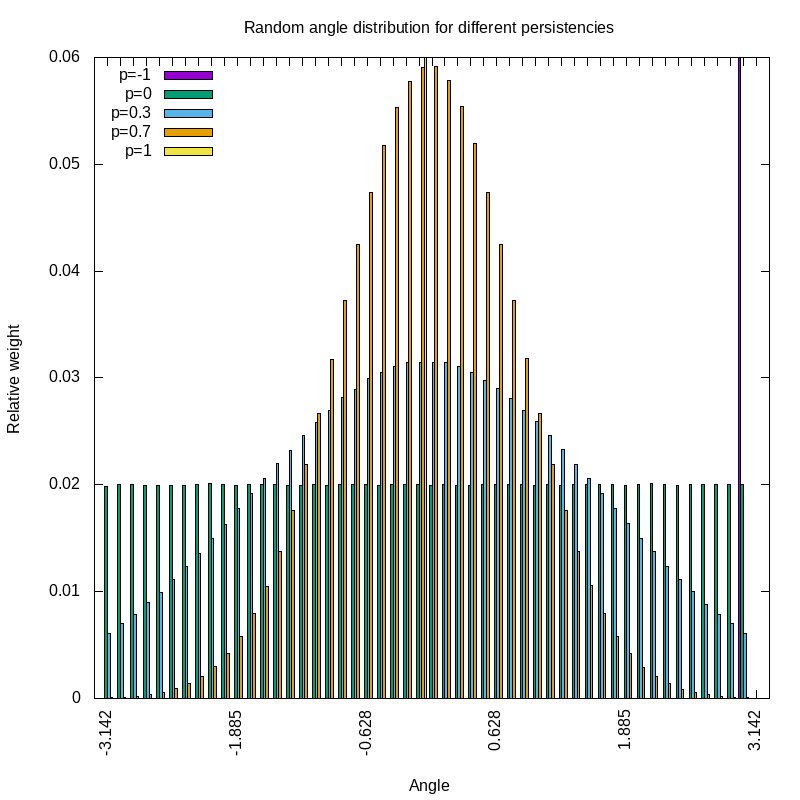
\includegraphics[width=0.8\textwidth]{./fig/cont/prep/angleDistribution.png}
 \caption{Distributions of generated random angles for different persistency parameters $p$.}
 \label{fig:cont-prep-angleDistribution}
\end{figure}

Another aspect worth looking at is the mean square displacement. Figure \ref{fig:cont-prep-msd} shows the mean square displacement for different values of p and therefore supports the fact that the walker is working as intended.

\begin{figure}[!hbt]
 \centering
 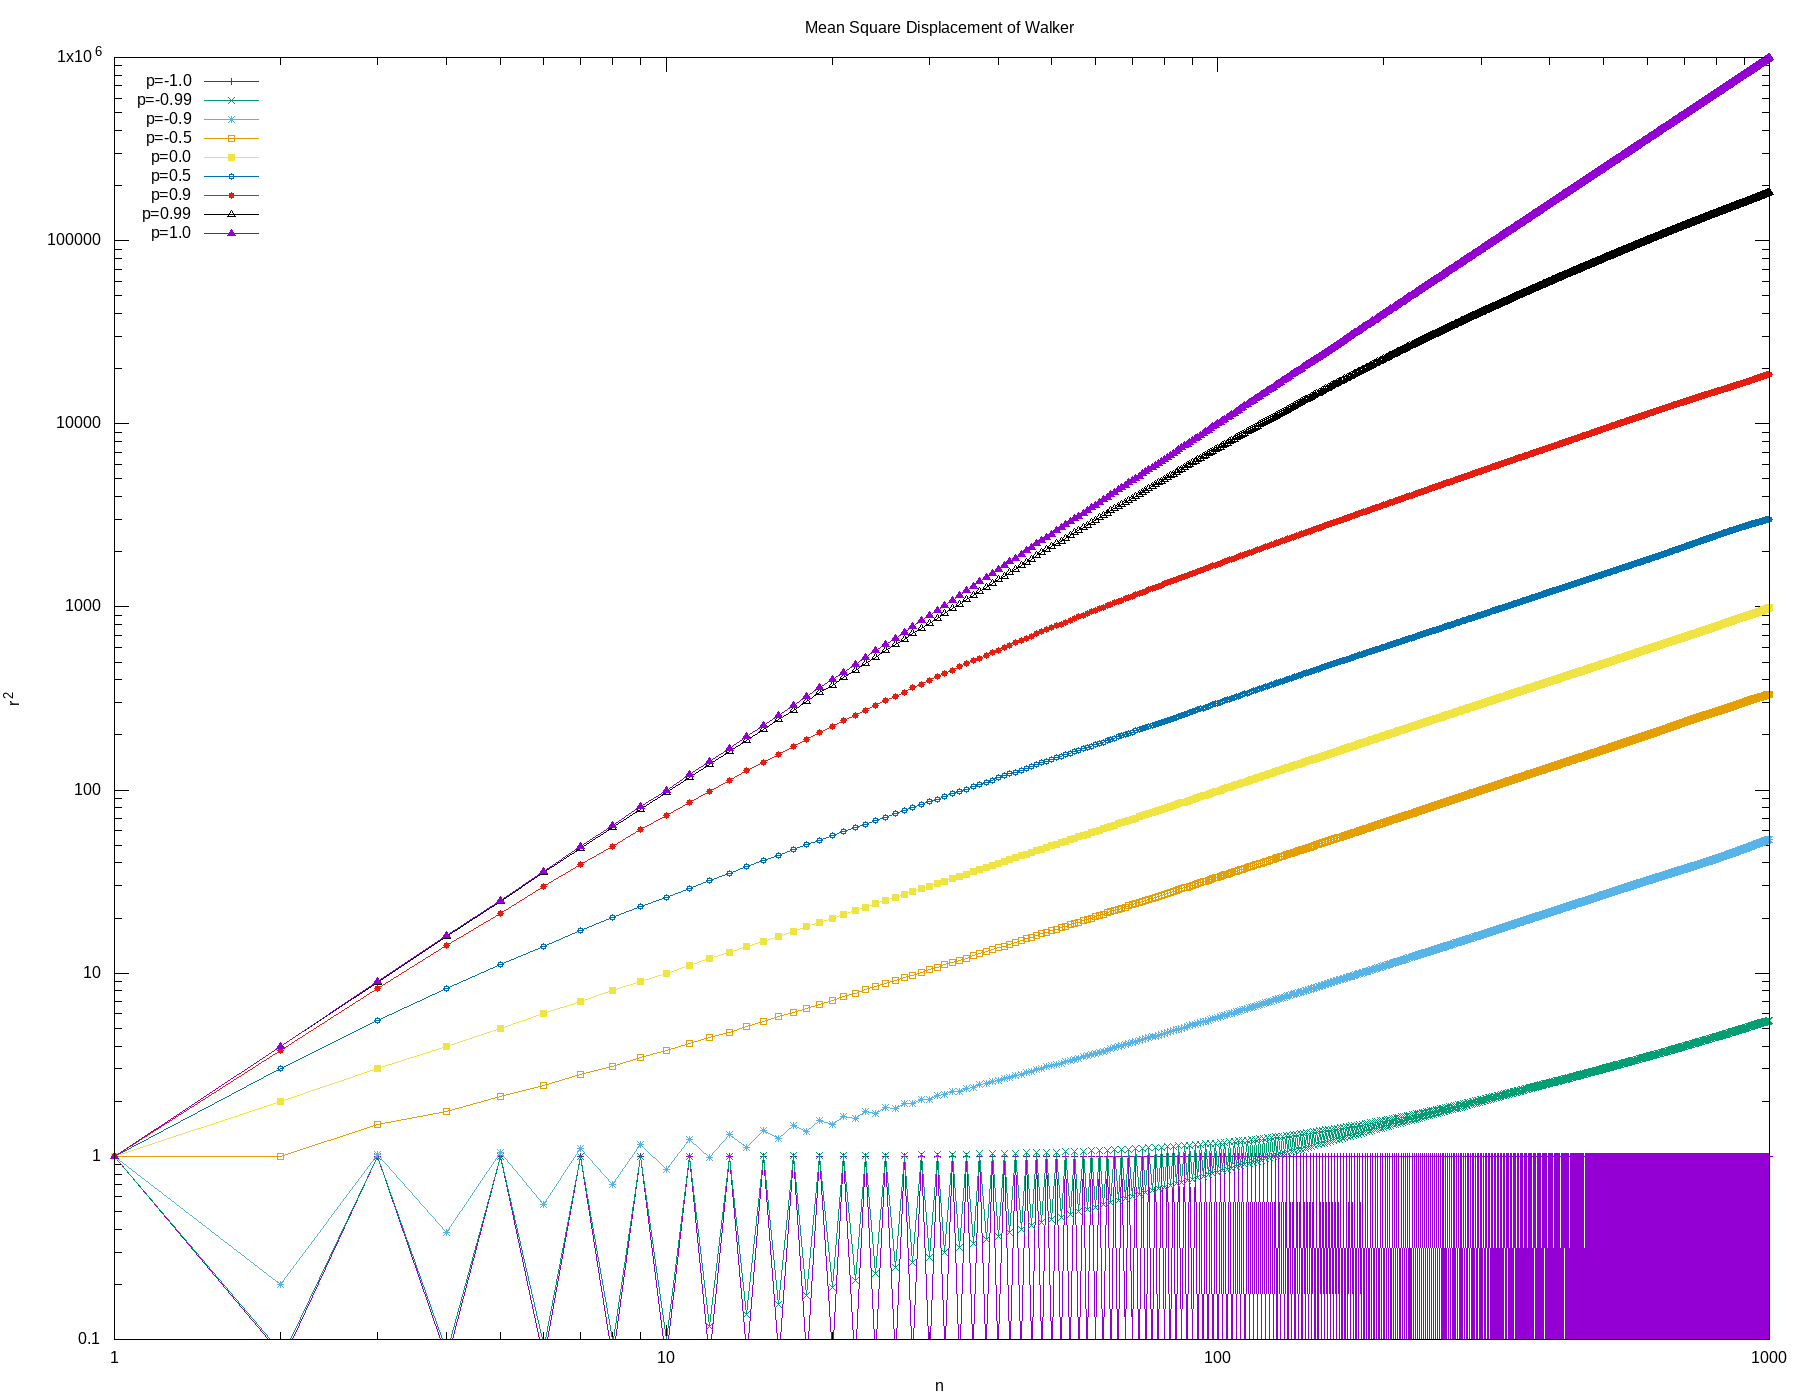
\includegraphics[width=0.8\textwidth]{./fig/cont/prep/msd-nruns=2000-nsteps=1000.png}
 \caption{Mean square displacement for different values of p averaged over 2000 runs with 1000 steps each.}
 \label{fig:cont-prep-msd}
\end{figure}

Since the persistent random walker is set now, one last question is over how many simulations one should average the mfpt simulations considering the statistical error and simulation time. From Figure xy one can see that 1e6 sample runs are sufficient considering that 1e7 runs would take a lot more time. Therefore, in the following results the mfpt averages are always taken over 1e6 samples. Also the starting position of the searcher is randomized for each single search.

TODO FIGURE NUMBER OF RUNS COMPARISON - WAITING FOR SIMULATIONS TO FINISH

\subsection{System length L}
\label{ssec:cont-L}

In order to get insight on the influence of the system length $L$ on the mean first passage time the system length has been varied between 10 and 1000.

TODO FIGURE SYSTEM LENGTH COMPARISON - WAITING FOR SIMULATIONS TO FINISH

\subsection{Detection radius D}
\label{ssec:cont-D}

Another aspect's influence on the mfpt that needs to be checked is the detection radius $D$ in which the walker finds the target. To do so the system length was fixed to $L = 200$ and the detection radius has been varied between 1 and 20 as can be seen in Figure xyz.

TODO FIGURE DETECTION RADIUS COMPARISON - WAITING FOR SIMULATIONS TO FINISH

\subsection{Deterministic approach}
\label{ssec:cont-deter}

One problem with above approach is the accuracy of the achieved persistency. Drawing random turning angles from the calculated distribution only gives the right persistency in the limit of drawing many angles, however searches with only a few thousand steps or even less tend to have slightly different overall persistency than the one that was given as input. Therefore a new approach is taken that is called the deterministic approach here even though it is not completely deterministic. Instead of drawing the turning angle from the calculated distribution as it was explained in subsection \ref{ssec:cont-prep} here one will simply use

\begin{equation}
 \label{eq:cont-deter-angle}
 \phi = \pm \arccos\left(p\right)
\end{equation}

where the only randomness is whether the walker turns left or right with equal probability. Using this approach it is ensured that the actual persistency is the input persistency $p$. Another positive aspect of this approach is that the simulation is faster.

Figure x and Figure y show the same simulation for system length and detection radius as above for this deterministic approach.

TODO FIGURE DETERMINISTIC COMPARISONS - WAITING FOR SIMULATIONS TO FINISH

\newpage

\section{Lattice Version}
\label{sec:latt}
In the lattice version of the program the persistency has a different meaning than in the continuous version. Here the persistency $p$ is the probability to keep going in the same direction as in the previous step whereas the other 3 directions are equally probable ($p_{left/right/back} = \frac{1 - p}{3}$).

So far for the lattice version the influence of the length of the system, the detection radius and absorbing walls on the mean first passage time have been examined. For all simulations the target has been centered and periodic boundary conditions were used except in the case of absorbing walls. Averages are taken over one million simulations as it was done in the continuous version.


\subsection{System length L}
\label{ssec:latt-L}

To examine the influence of the system length on the mean first passage time the system length has been varied between 10 and 1000 lattice sites.

\begin{figure}[!hbt]
 \centering
 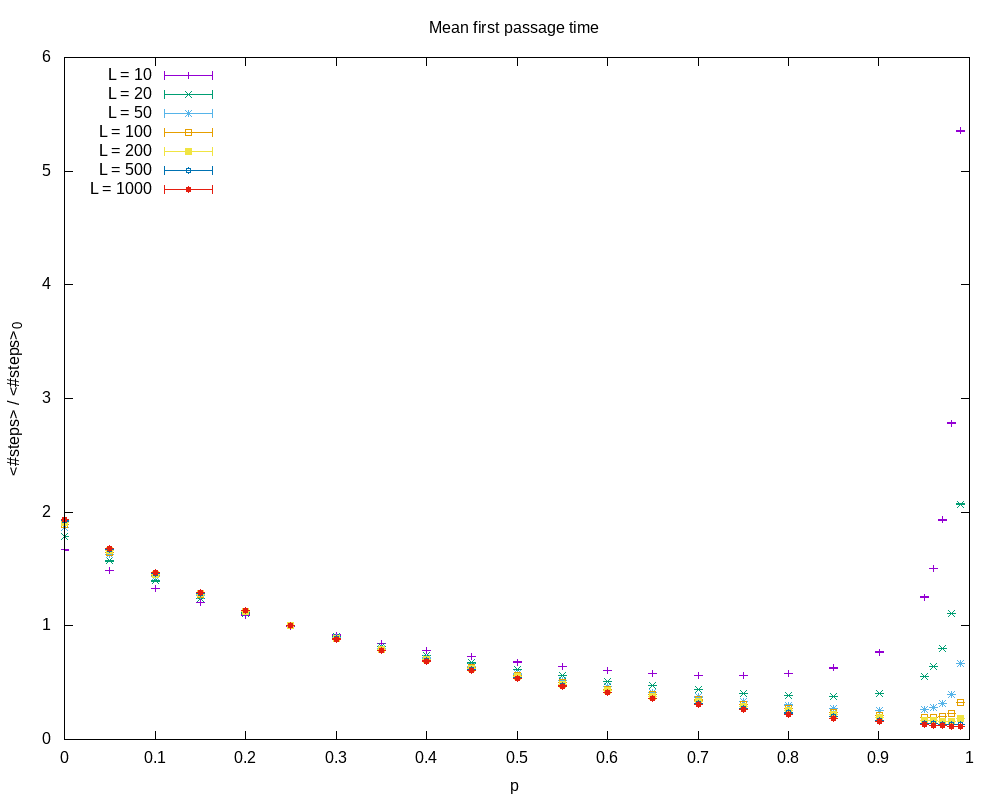
\includegraphics[width=0.8\textwidth]{./fig/latt/L/fpt.png}
 \caption{Mean first passage time in dependency on the persistency for different system lengths. Mean first passage time has been rescaled by the mean first passage time for $p = 0.25$ which corresponds to diffusion.}\label{fig:latt-L-fpt}
\end{figure}

As one can see in Figure \ref{fig:latt-L-fpt} the minimum of the mean first passage time shifts to higher values of p (higher persistency) as the system length increases. Figure \ref{fig:latt-L-p_opt} shows this more clearly and gives reason to assume that the optimal persistency approaches 1 in the limit of huge system sizes.

\begin{figure}[!hbt]
 \centering
 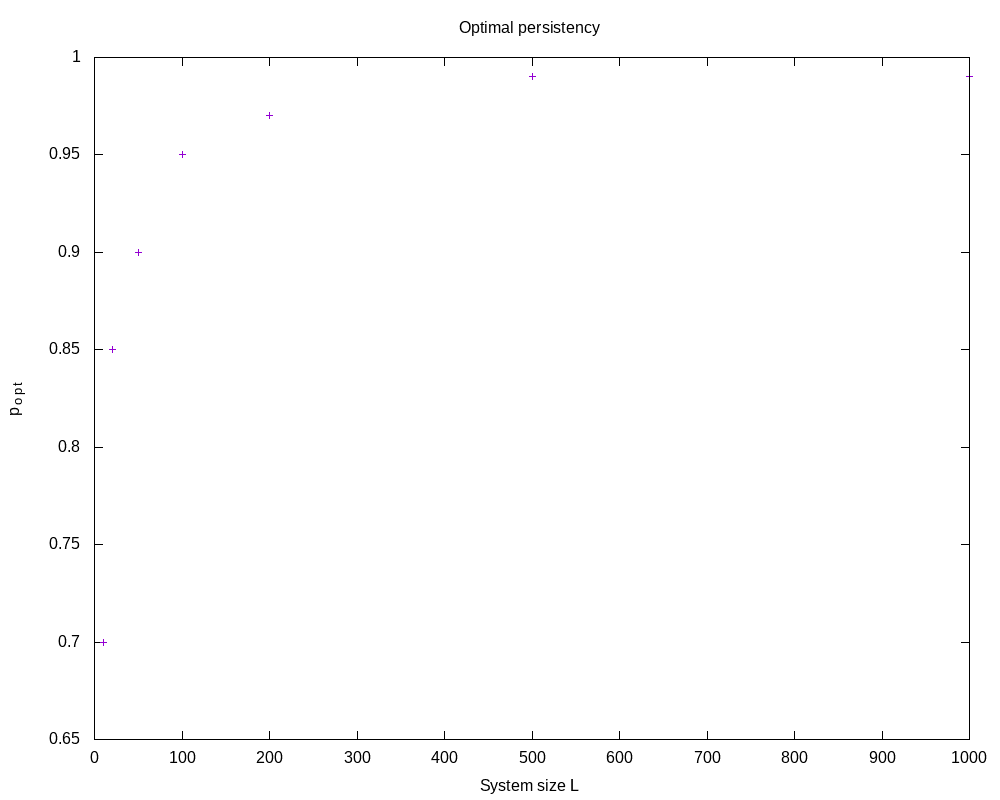
\includegraphics[width=0.8\textwidth]{./fig/latt/L/p_opt.png}
 \caption{Optimal persistency in dependency on the system length.}
 \label{fig:latt-L-p_opt}
\end{figure}

Furthermore, figure \ref{fig:latt-L-p_opt-logscales} shows different logscales for the optimal persistency to prove that there is no easy mathematical law describing the dependency.
 
 \begin{figure}[!hbt]
\centering
% \captionsetup[subfigure]{justification=justified,singlelinecheck=false,labelformat=simple}
\begin{subfigure}{0.35\textwidth}
 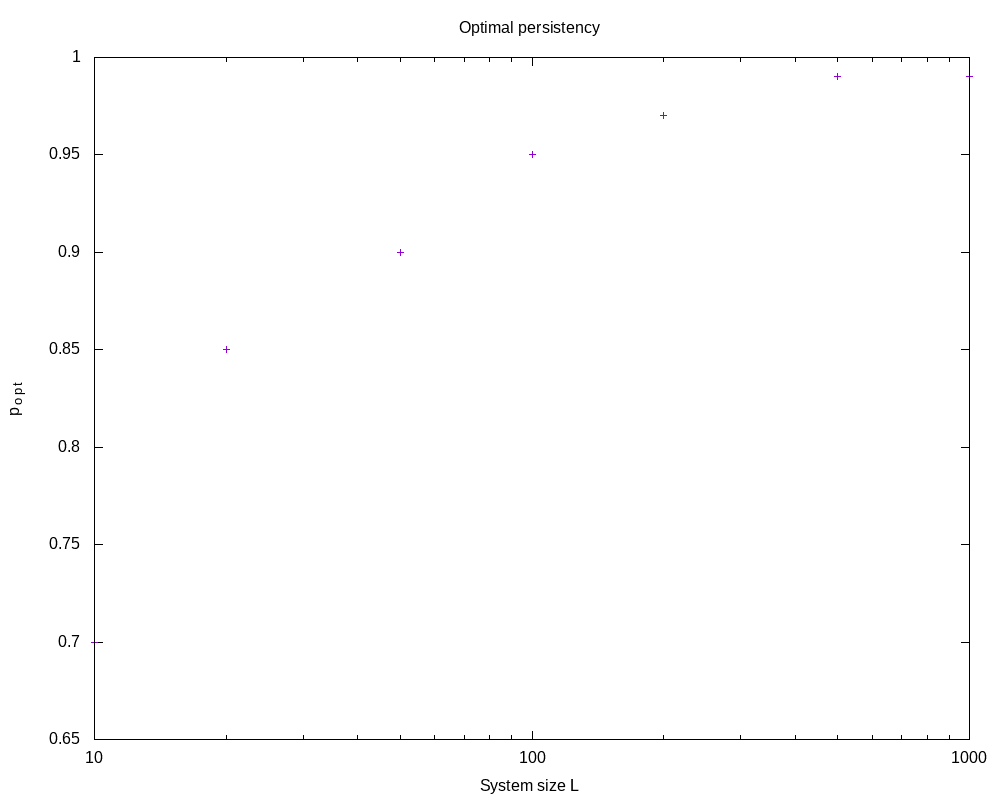
\includegraphics[width=\textwidth]{./fig/latt/L/p_opt_logx.png}
  \subcaption{x logscale}
%  \label{}
\end{subfigure}
\begin{subfigure}{0.35\textwidth}
 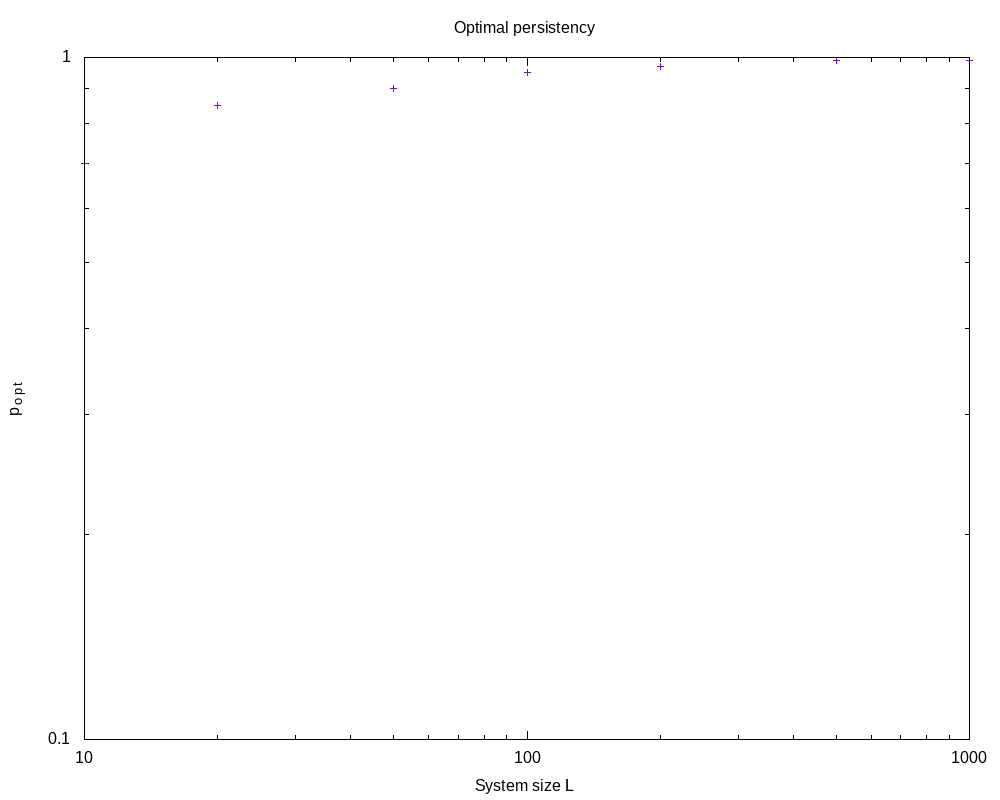
\includegraphics[width=\textwidth]{./fig/latt/L/p_opt_logxy.png}
  \subcaption{xy logscale}
%  \label{}
\end{subfigure}
\begin{subfigure}{0.35\textwidth}
 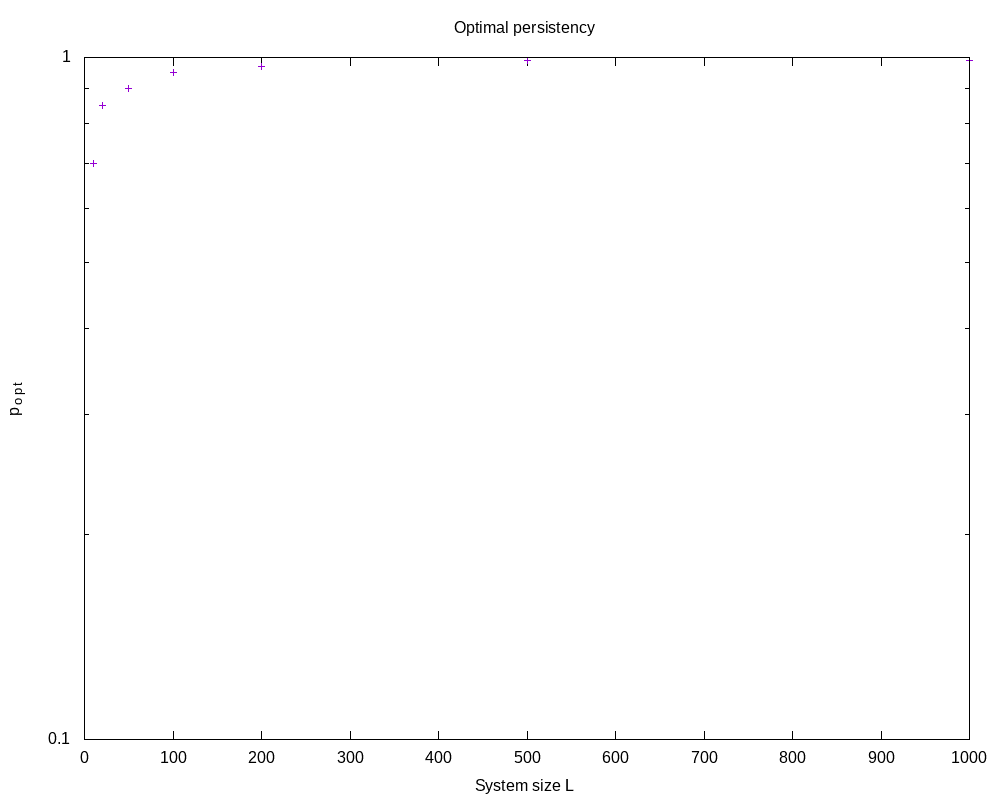
\includegraphics[width=\textwidth]{./fig/latt/L/p_opt_logy.png}
  \subcaption{y logscale}
%  \label{}
\end{subfigure}
\caption{Different logscales for the optimal persistency in dependency on the system length.} 
\label{fig:latt-L-p_opt-logscales}
\end{figure}


\subsection{Detection Radius D}
\label{ssec:latt-D}

In order to check on the influence of the detection radius on the first passage time the system length has been chosen to be $L = 200$ and the detection radius has been varied between 1 and 20.

\begin{figure}[!hbt]
 \centering
 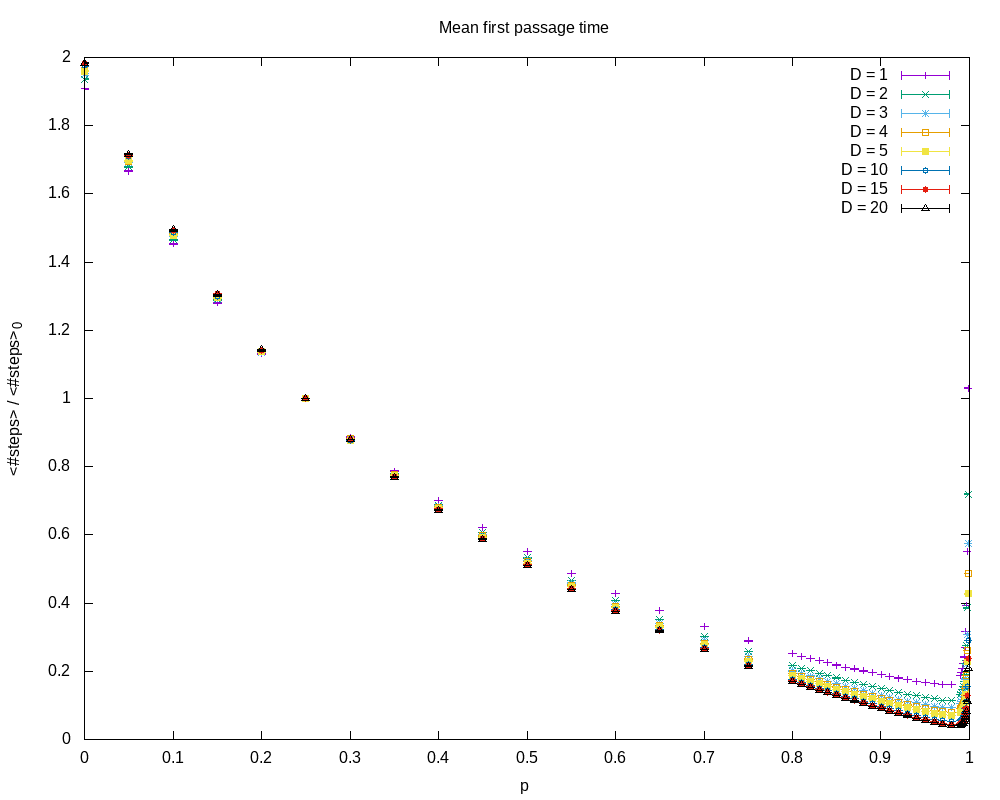
\includegraphics[width=0.8\textwidth]{./fig/latt/D/fpt.png}
 \caption{Mean first passage time in dependency on the persistency for different detection radii. Mean first passage time has been rescaled by the mean first passage time for $p = 0.25$ which corresponds to diffusion.\label{fig:latt-D-fpt}}
\end{figure}

The persistency value at the minimum of the mean first passage time seems to be unaffected by changes to the detection radius as can be seen in Figure \ref{fig:latt-D-fpt} and Figure \ref{fig:latt-D-opt_p}.

\begin{figure}[!hbt]
 \centering
 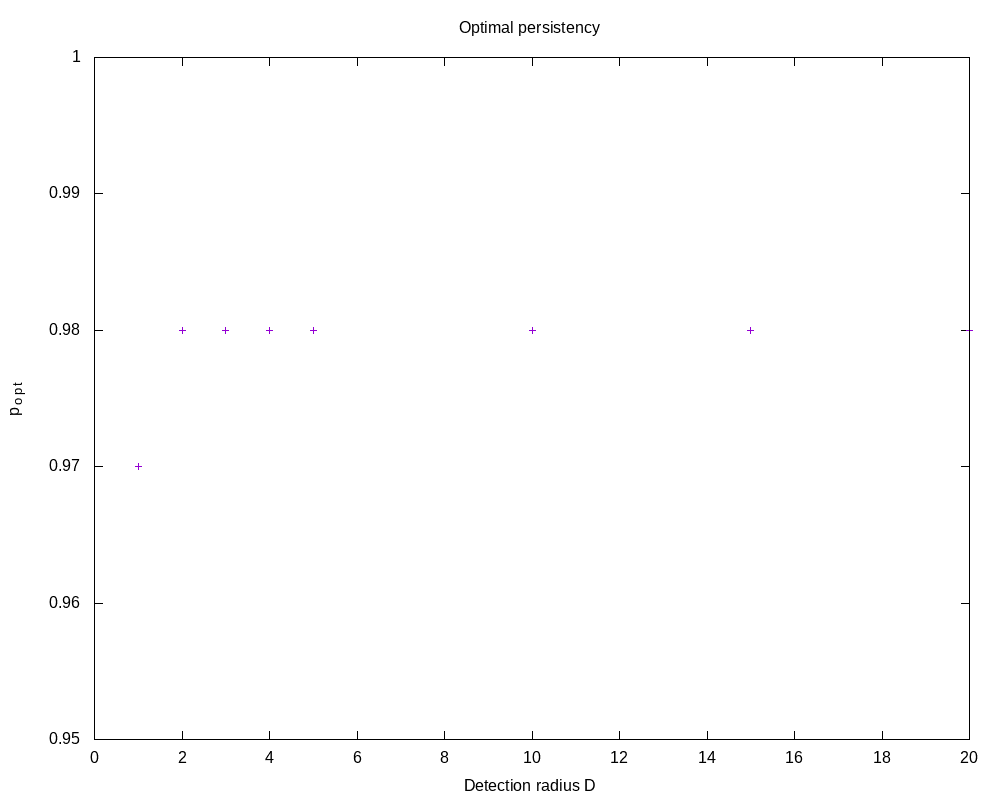
\includegraphics[width=0.8\textwidth]{./fig/latt/D/p_opt.png}
 \caption{Optimal persistency in dependency on the detection radius.}
 \label{fig:latt-D-opt_p}
\end{figure}


\subsection{Absorbing boundaries}
\label{ssec:latt-alpha}

A third property to consider were the boundary conditions of the system. So far periodic boundaries have been examined. On the following pages the results of absorbing boundary conditions will be shown. Therefore, a new parameter $\alpha$ is introduced, which gives the probability of the searcher to be released from the absorbing wall in each timestep. Also the influence of the system length for absorbing boundaries will be shown. However, the detection radius is fixed to $D = 1$ in the following. The position of the target is also randomized for each single simulation.

 \begin{figure}[!hbt]
\centering
% \captionsetup[subfigure]{justification=justified,singlelinecheck=false,labelformat=simple}
\begin{subfigure}{0.45\textwidth}
 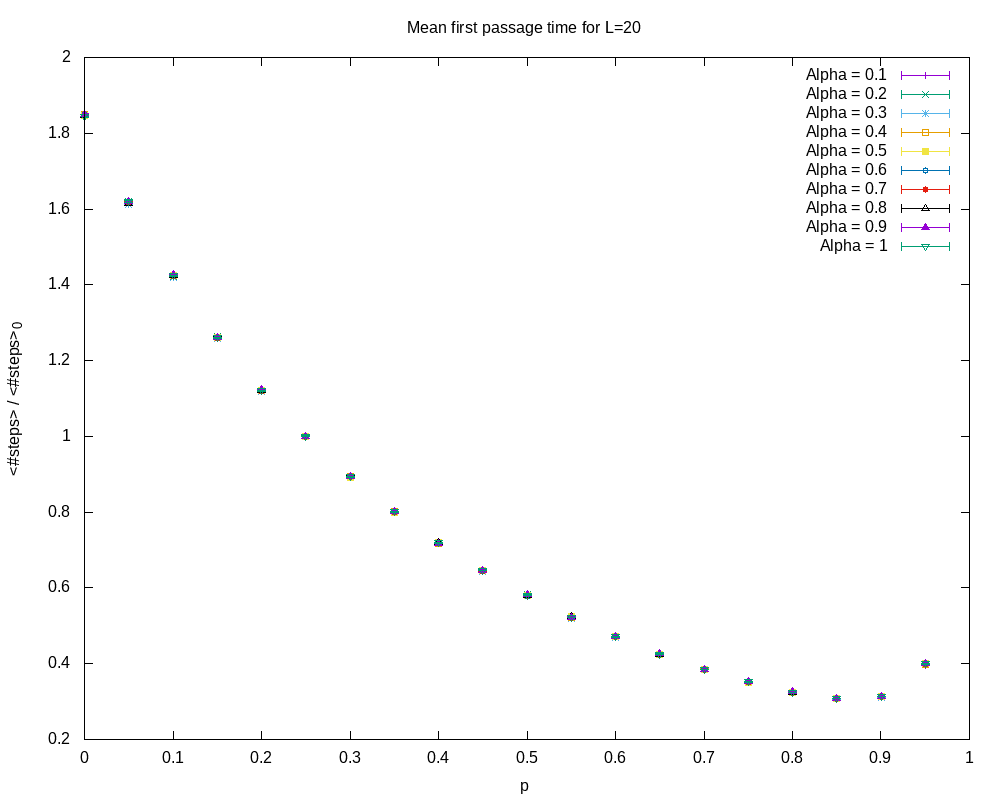
\includegraphics[width=\textwidth]{./fig/latt/alpha/L=20/fpt.png}
  \subcaption{Rescaled MFPT}
%  \label{}
\end{subfigure}
\begin{subfigure}{0.45\textwidth}
 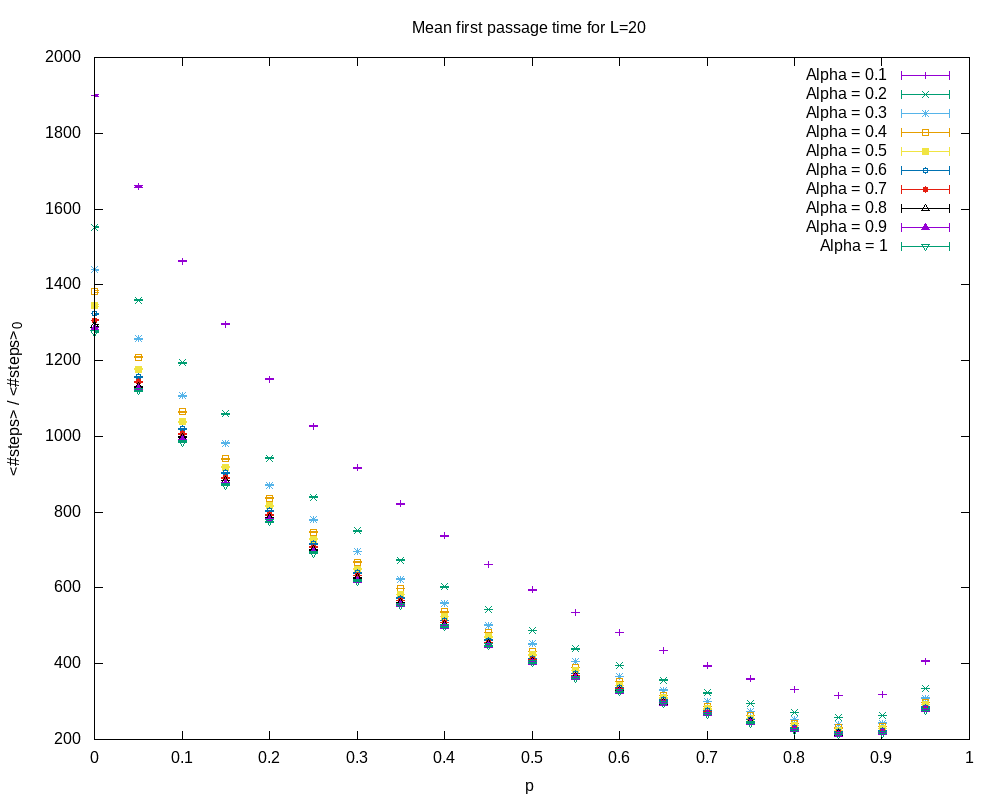
\includegraphics[width=\textwidth]{./fig/latt/alpha/L=20/fpt2.png}
  \subcaption{MFPT}
%  \label{}
\end{subfigure}
\caption{Mean first passage time for system length $L = 20$ and absorbing boundary conditions for different parameters $\alpha$. (a) Mean first passage time rescaled by mfpt for $p = 0.25$. (b) Unscaled mfpt.} 
\label{fig:latt-alpha-fpts20}
\end{figure}

 \begin{figure}[!hbt]
\centering
% \captionsetup[subfigure]{justification=justified,singlelinecheck=false,labelformat=simple}
\begin{subfigure}{0.45\textwidth}
 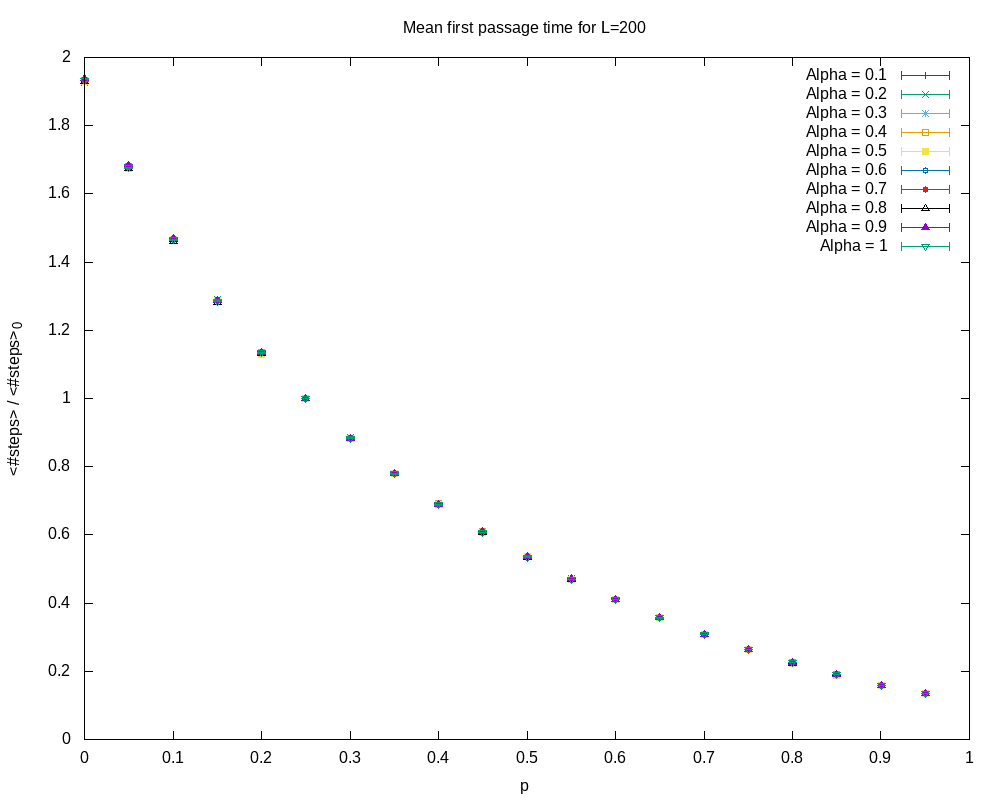
\includegraphics[width=\textwidth]{./fig/latt/alpha/L=200/fpt.png}
  \subcaption{Rescaled MFPT}
%  \label{}
\end{subfigure}
\begin{subfigure}{0.45\textwidth}
 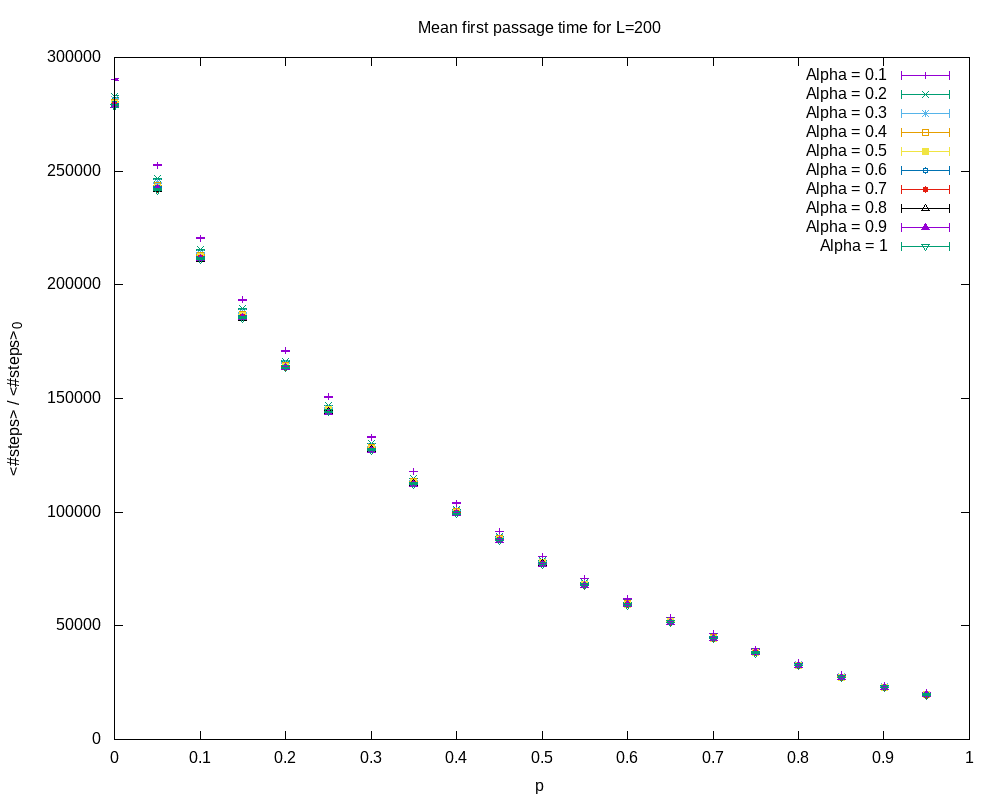
\includegraphics[width=\textwidth]{./fig/latt/alpha/L=200/fpt2.png}
  \subcaption{MFPT}
%  \label{}
\end{subfigure}
\caption{Mean first passage time for system length $L = 200$ and absorbing boundary conditions for different parameters $\alpha$. (a) Mean first passage time rescaled by mfpt for $p = 0.25$. (b) Unscaled mfpt.} 
\label{fig:latt-alpha-fpts200}
\end{figure}

As shown in Figure \ref{fig:latt-alpha-fpts20} and Figure \ref{fig:latt-alpha-fpts200} the influence of different system lengths is not altered in comparison to periodic boundary conditions (compare Figure \ref{fig:latt-L-fpt}). Additionally, the variation of the parameter $\alpha$ does not influence the position of the optimal persistency at all. At first this is unexpected as one could assume that low $\alpha$ corresponds to long waiting times on the walls and therefore avoiding the walls would be beneficial. To gain further insight into this property, Figure \ref{fig:latt-alpha-wallFreq} shows the average frequency of wall hits per step in a system of length $L = 200$ taken over one billion steps for three different values $\alpha$.

 \begin{figure}[!hbt]
\centering
% \captionsetup[subfigure]{justification=justified,singlelinecheck=false,labelformat=simple}
\begin{subfigure}{0.45\textwidth}
 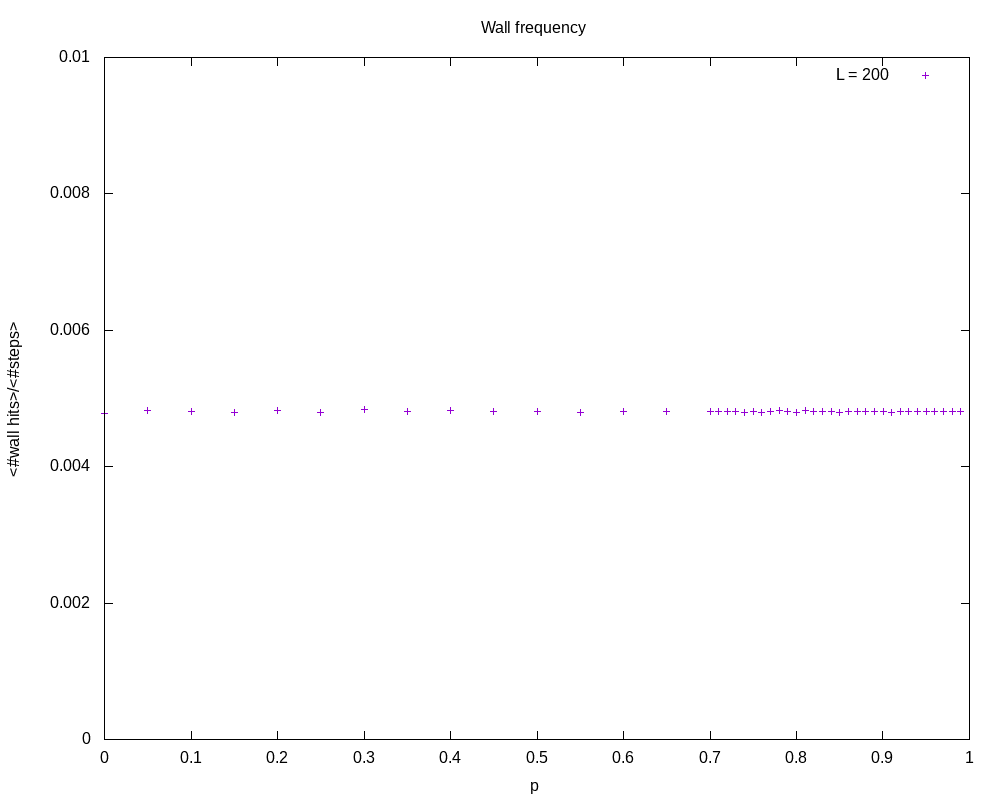
\includegraphics[width=\textwidth]{./fig/latt/alpha/wallFreq/WF-alpha=01-rel.png}
  \subcaption{$\alpha = 0.1$}
%  \label{}
\end{subfigure}
\begin{subfigure}{0.45\textwidth}
 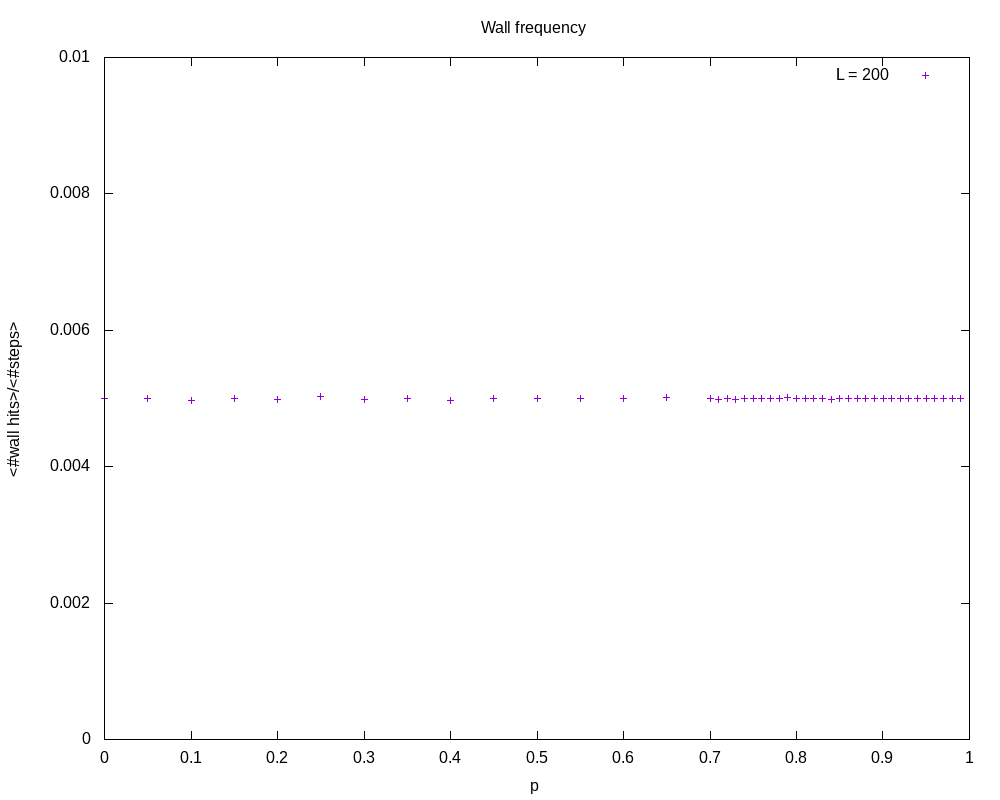
\includegraphics[width=\textwidth]{./fig/latt/alpha/wallFreq/WF-alpha=05-rel.png}
  \subcaption{$\alpha = 0.5$}
%  \label{}
\end{subfigure}
\begin{subfigure}{0.45\textwidth}
 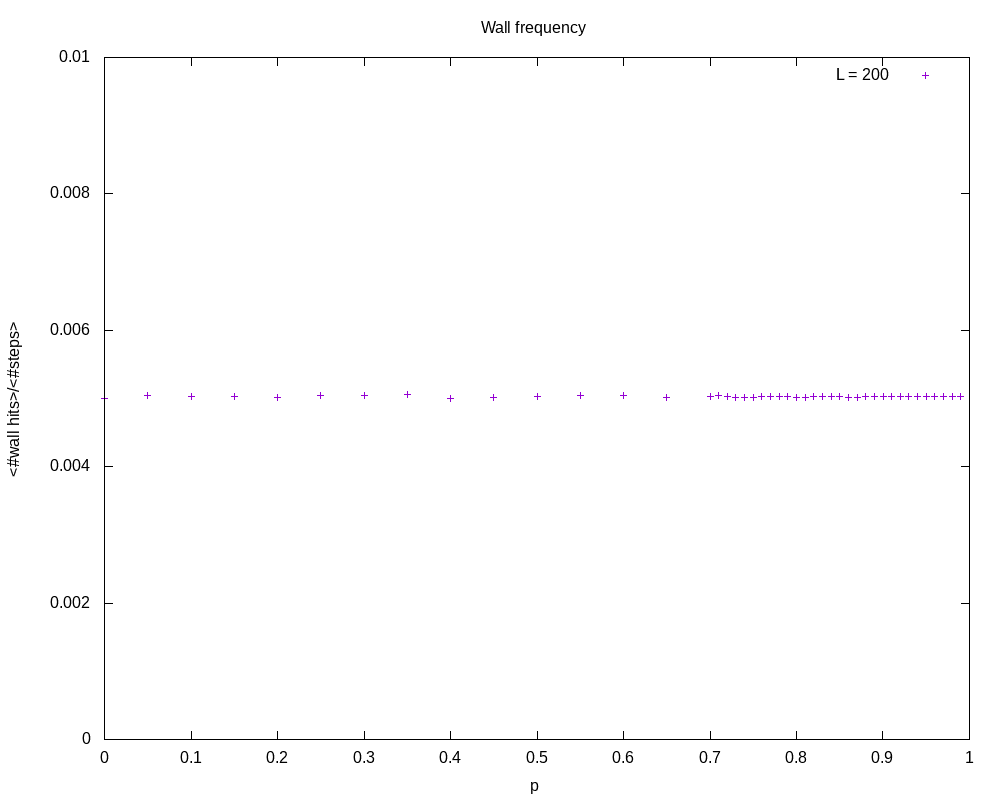
\includegraphics[width=\textwidth]{./fig/latt/alpha/wallFreq/WF-alpha=1-rel.png}
  \subcaption{$\alpha = 1$}
%  \label{}
\end{subfigure}
\caption{Wall hit frequency per step for different values of $\alpha$ in a system of length $L = 200$.} 
\label{fig:latt-alpha-wallFreq}
\end{figure}

With Figure \ref{fig:latt-alpha-wallFreq} the results of Figure \ref{fig:latt-alpha-fpts20} and Figure \ref{fig:latt-alpha-fpts200} can be understood. As the amount of timesteps spent on the walls does not depend on the persistency but only on the total amount of time spent in the system, it is clear that the optimal persistency will remain the same when changing periodic boundaries to absorbing boundaries. The minimum will be even more clear in the case of absorbing boundaries since the smallest mfpt corresponds to lowest amount of timesteps spent on walls.

%  \begin{figure}[b]
%  \centering
%  \includegraphics[width=1.0\textwidth]{Figure1.eps}
%  \caption{aaa.}
%  \label{Fig1}
%  \end{figure} 
 

\end{document}
